\documentclass{beamer}

\mode<presentation> {
% Colors

%\usetheme{default}
%\usetheme{AnnArbor}
%\usetheme{Antibes}
%\usetheme{Bergen}
%\usetheme{Berkeley}
%\usetheme{Berlin}
%\usetheme{Boadilla}
%\usetheme{CambridgeUS}
%\usetheme{Copenhagen}
%\usetheme{Darmstadt}
%\usetheme{Dresden}
%\usetheme{Frankfurt}
%\usetheme{Goettingen}
%\usetheme{Hannover}
\usetheme{Ilmenau}
%\usetheme{JuanLesPins}
%\usetheme{Luebeck}
%\usetheme{Madrid}
%\usetheme{Malmoe}
%\usetheme{Marburg}
%\usetheme{Montpellier}
%\usetheme{PaloAlto}
%\usetheme{Pittsburgh}
%\usetheme{Rochester}
%\usetheme{Singapore}
%\usetheme{Szeged}
%\usetheme{Warsaw}

%Themes

%\usecolortheme{albatross}
%\usecolortheme{beaver}
%\usecolortheme{beetle}
%\usecolortheme{crane}
%\usecolortheme{dolphin}
%\usecolortheme{dove}
%\usecolortheme{fly}
%\usecolortheme{lily}
%\usecolortheme{orchid}
%\usecolortheme{rose}
%\usecolortheme{seagull}
%\usecolortheme{seahorse}
%\usecolortheme{whale}
%\usecolortheme{wolverine}

%\setbeamertemplate{footline} % To remove the footer line in all slides uncomment this line
%\setbeamertemplate{footline}[page number] % To replace the footer line in all slides with a simple slide count uncomment this line

\setbeamertemplate{navigation symbols}{} % To remove the navigation symbols from the bottom of all slides uncomment this line
}

\usepackage{graphicx} % Allows including images
\usepackage{booktabs} % Allows the use of \toprule, \midrule and \bottomrule in tables

%----------------------------------------------------------------------------------------
%	TITLE PAGE
%----------------------------------------------------------------------------------------

\title[NMR Assignment with A*]{Accelerating Biomolecular Nuclear Magnetic Resonance Assignment with A*} % The short title appears at the bottom of every slide, the full title is only on the title page

\author[J. Venzke, P. Johnson, R. Davis, J. Emmons, K. Roth, D. Mascharka, L. Robison, T. Urness, A. Kilpatrick]{Joel Venzke, Paxten Johnson, Rachel Davis, John Emmons,\\ Katherine Roth, David Mascharka, Leah Robison,\\ Timothy Urness and Adina Kilpatrick} % Your name
\institute[Drake University] % Your institution as it will appear on the bottom of every slide, may be shorthand to save space
{
Department of Mathematics and Computer Science\\
Drake University\\

\medskip
\textit{joel.venzke@drake.edu} % Your email address
}
\date{April 10,2014} % Date, can be changed to a custom date

\begin{document}

\begin{frame}
\titlepage % Print the title page as the first slide
\end{frame}

% =======================================================================
% =======================================================================
\section{Introduction}
\begin{frame}
\frametitle{Overview} % Table of contents slide, comment this block out to remove it
\tableofcontents 
\end{frame}

\subsection{Motivation} 
\begin{frame}
	\frametitle{Title}
	\begin{itemize}
		\item Nuclear Magnetic Resonance Spectroscopy
		\begin{itemize}
			\item Gain knowledge protein structure
			\item Study how mutations lead to diseases
		\end{itemize}
		\item Problems
		\begin{itemize}
			\item Generators large amounts of data
			\item Data analysis it slow and error prone 
		\end{itemize}
		\item Goal
		\begin{itemize}
			\item automate the assignment process
			\item decrease human error
			\item increase productivity
		\end{itemize}
	\end{itemize}
\end{frame}

% =======================================================================
\subsection{Nuclear Magnetic Resonance Spectroscopy} 
\begin{frame}
	\frametitle{Nuclear Magnetic Resonance (NMR)}
	\begin{itemize}
		\item 
	\end{itemize}
\end{frame}

\begin{frame}
	\frametitle{Chemical Shift Values}
	\begin{figure}[H]
	\begin{center}
	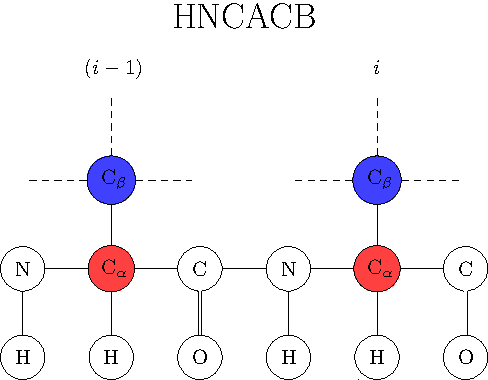
\includegraphics[width=.65\textwidth]{diagram}
	\end{center}
	\end{figure}
\end{frame}



% =======================================================================
% =======================================================================
\section{Assignment Process}

% =======================================================================
\subsection{Data Collection}
\begin{frame}
	\frametitle{Data Collection Time Line}
	\begin{itemize}
		\item Protein production
		\begin{itemize}
			\item At least 5 days \cite{babak_alipanahi_error_2011}
		\end{itemize}
		\item NMR Experiments 
		\begin{itemize}
			\item 1 to 2 days per spectrum involved \cite{babak_alipanahi_error_2011}
		\end{itemize}
		\item Assignment can begin
	\end{itemize}
	
\end{frame}

% =======================================================================
\subsection{Manual Assignment}
\begin{frame}
	\frametitle{Manual Methods}
	\begin{itemize}
		\item 
	\end{itemize}

\end{frame}


% =======================================================================
% =======================================================================
\section{Automation Algorithm}

% =======================================================================
\subsection{Preprocessing}

\begin{frame}
	\frametitle{Initialization}
	\begin{itemize}
		\item Input
		\begin{itemize}
			\item Expected amino acid sequence
			\begin{itemize}
				\item Covered to expectation chemical shift values
				\item Stored as the protein chain
			\end{itemize}
			\item NMR chemical shift data
			\begin{itemize}
				\item $C_\alpha$ and $C_{\beta}$ for residue $i$ and $i-1$
				\item Stored in a tile
			\end{itemize}
		\end{itemize}
		\item Missing data
		\begin{itemize}
			\item Place holder tile generation
		\end{itemize}
		\item Grouping 
	\end{itemize}
\end{frame}

\begin{frame}
	\frametitle{Grouping}
	\begin{figure}[H]
	\begin{center}
	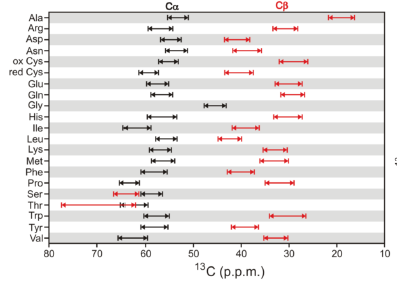
\includegraphics[width=.65\textwidth]{carbon}
	\end{center}
	\end{figure}
\cite{carbon}
\end{frame}

% =======================================================================
\subsection{Assignment}

\begin{frame}
	\frametitle{Title}
	\begin{itemize}
		\item 
	\end{itemize}
\end{frame}


% =======================================================================
% =======================================================================
\section{Conclusion}

% =======================================================================
\subsection{Results}

\begin{frame}
	\frametitle{Time of Assignment}
	\begin{figure}[H]
	\begin{center}
	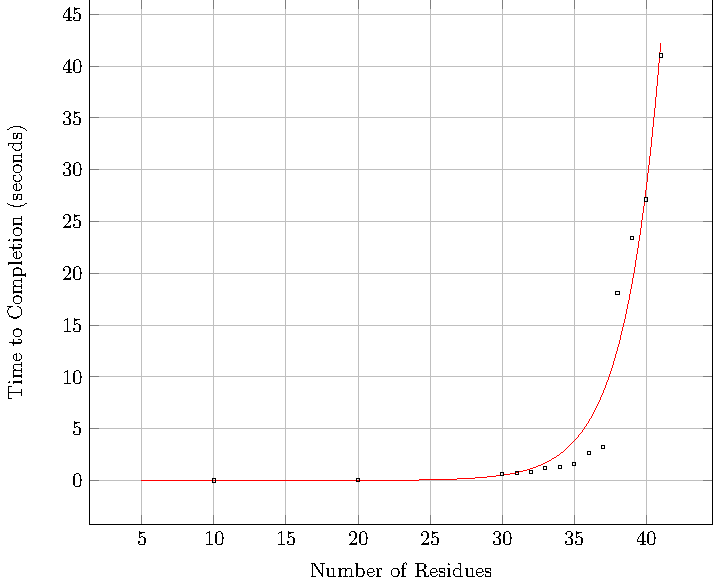
\includegraphics[width=.65\textwidth]{plot}
	\end{center}
	\end{figure}
\end{frame}

\begin{frame}
	\frametitle{Assignment Issues}
	\begin{itemize}
		\item Missing data decreases accuracy
		\begin{itemize}
			\item increases assignment time
		\end{itemize}
	\end{itemize}
\end{frame}



% =======================================================================
\subsection{Outlook}
\begin{frame}
	\frametitle{Future Goals}
	\begin{itemize}
		\item Parallelization
		\begin{itemize}
			\item Decrease assignment time
			\item Allow for lager data sets
		\end{itemize}
		\item Machine learning 
		\begin{itemize}
			\item Increase accuracy of assignment
			\item Optimize cost calculation
		\end{itemize}
	\end{itemize}
\end{frame}


\begin{frame}{Bibliography}
\bibliographystyle{amc}
\bibliography{presentaion}
\end{frame}
\end{document}